%%
%% Author: novitoll
%% 2/25/18
%%

% Preamble
\documentclass[11pt]{article}

% Packages
\usepackage{graphicx}
\usepackage{amsmath}
\usepackage{hyperref}

\title{CVT: Lecture 4}
\date{2018-02-25}
\author{Novitoll}

\graphicspath{ {code/} }

% Document
\begin{document}

    \section{Hough space}

    In short, Hough space is the interpretation of (x, y, ..) coordinates' \textit{a, slope} and
    \textit{b, intercept},
    for $y = ax + b$ linear function, e\.g\.:

    \begin{itemize}
        \item point in Cartesian coordinate - line in Hough space
        \item line in Cartesian coordinate - point in Hough space
    \end{itemize}

    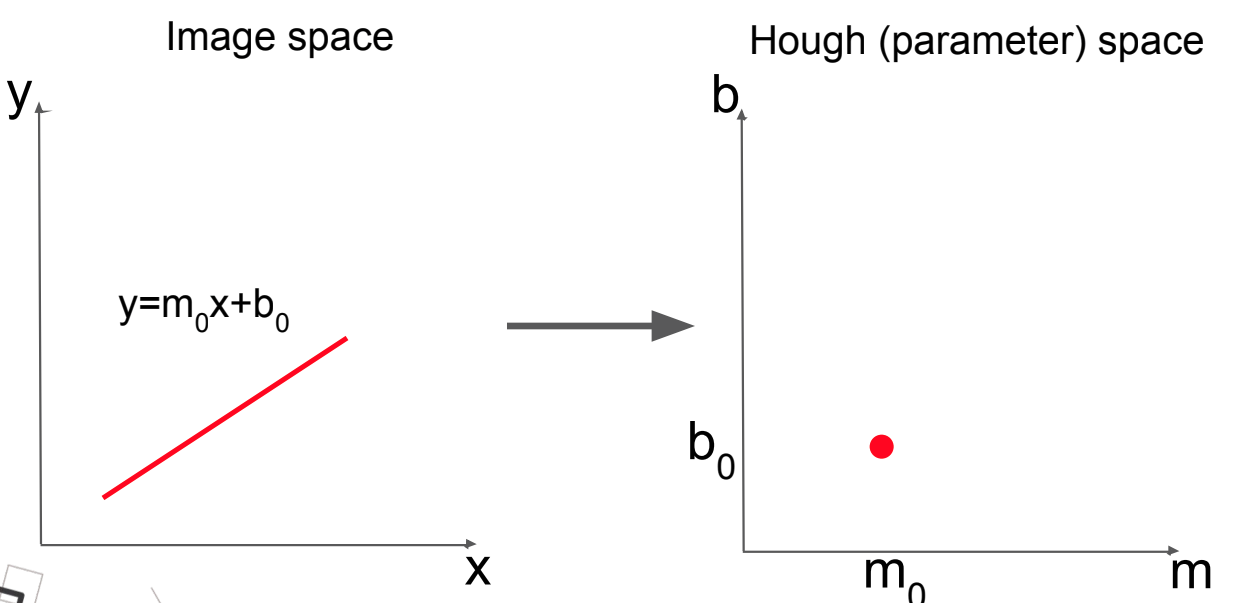
\includegraphics[scale=0.2]{hough_space}

    However, in Cartesian coordinate system there is a problem for Hough space:

    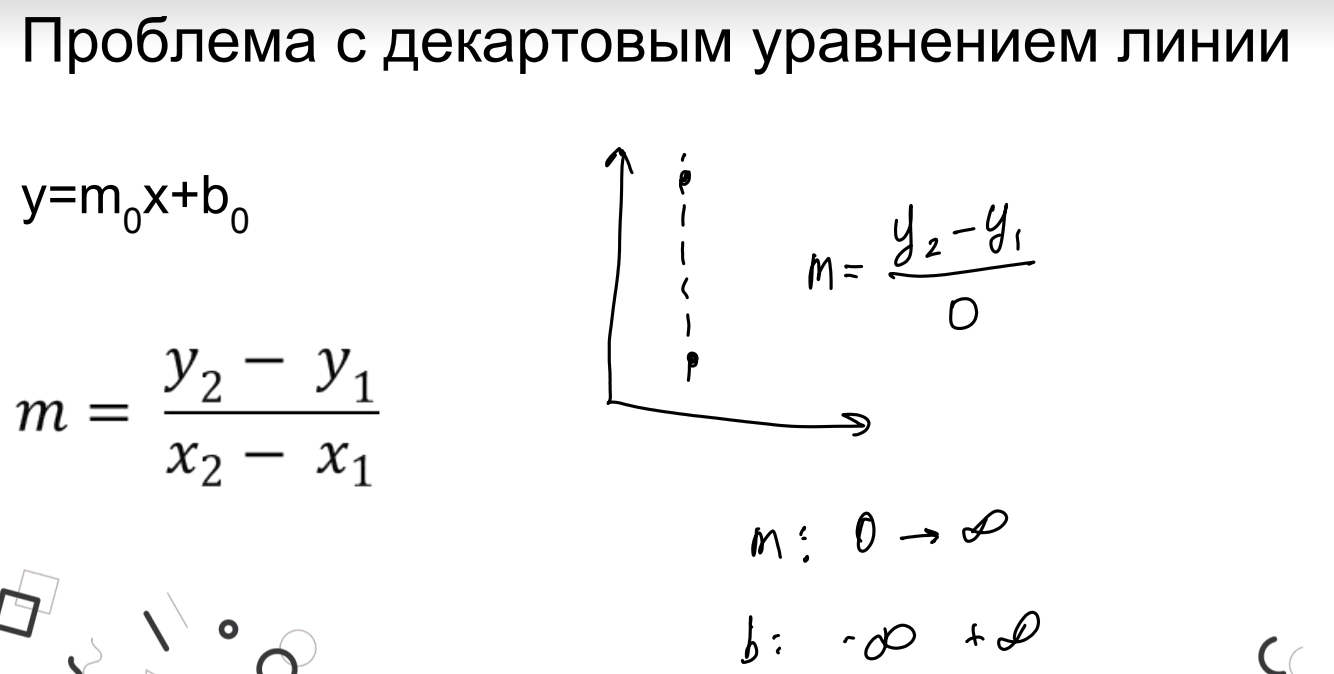
\includegraphics[scale=0.2]{cartesian_problem}

    to solve this issue, the same coordinates can be transformed to \emph{polar system coordinate}

    \begin{align}
        \rho &= x * cos(\theta) + y * cos(\theta)
    \end{align}

    , where in this case, the angle $\theta : 0 - 180^0$.


    So with polar system coord\. Hough space is:

    \begin{itemize}
        \item point in image, sinusoid in Hough space
    \end{itemize}

    The result of Hough space in polar system is the \textbf{Hough accumulator},
    which is the 2D array of $\rho$ and $\theta$

    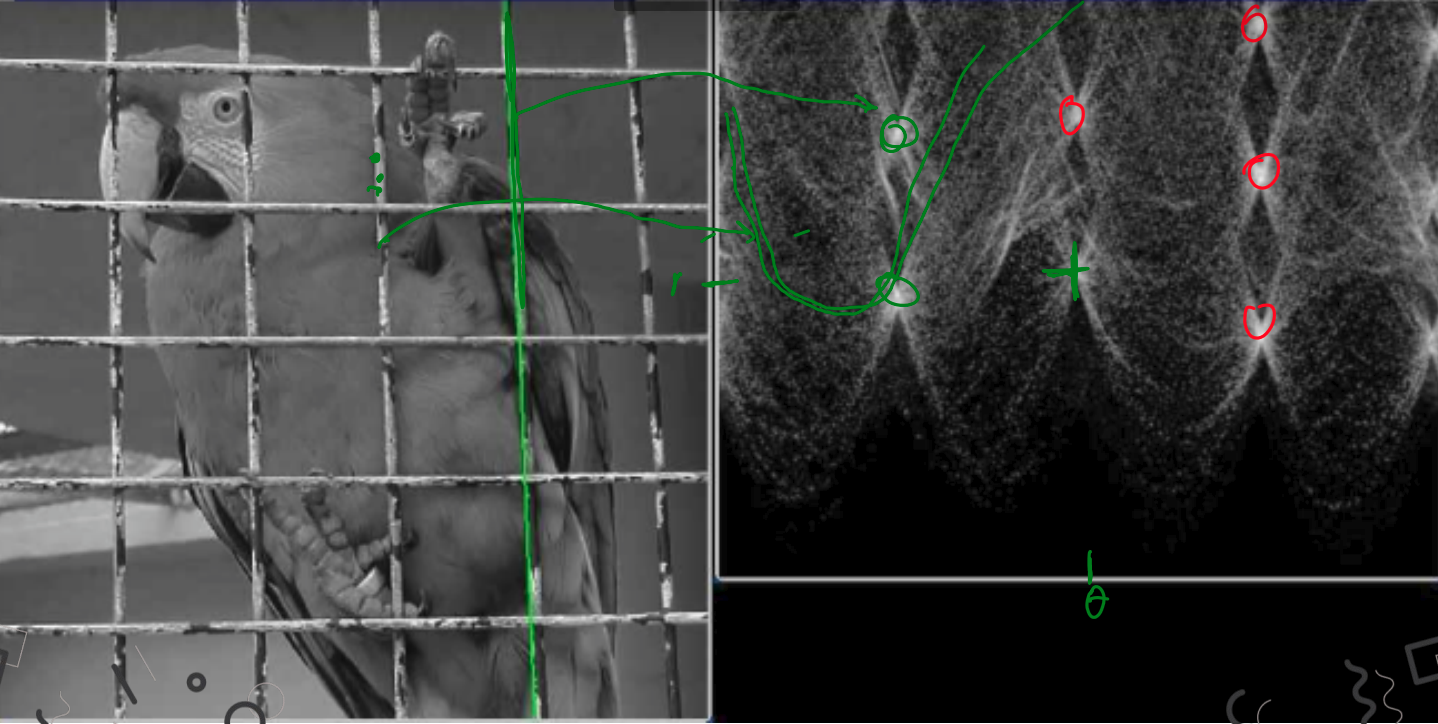
\includegraphics[scale=0.2]{hough_space_lines}

    \section{PClines}

    \href{CVPR 2011}{https://www.youtube.com/watch?v=ZAJFnafV3oo}:
    "Line detection by Hough transform based on parameterization using parallel coordinates."

    In short, interpret Cartesian (x, y, ..) coordinates in Parallel system coordinate
    (with additional inverse \textbf{y} axis (watch video above to see the reason)) and work there with Hough transform

    \section{Canny algorithm (edge detector)}

    In short, Canny uses 2 thresholds $ C_1, C_2 $
    where $ C_1 < C_2 $, then
    it detects strong gradients bigger than $ C_1 $,
    proceed with the gradient, rather than filtering
    until it limits to the lower $ C_2 $ threshold.

    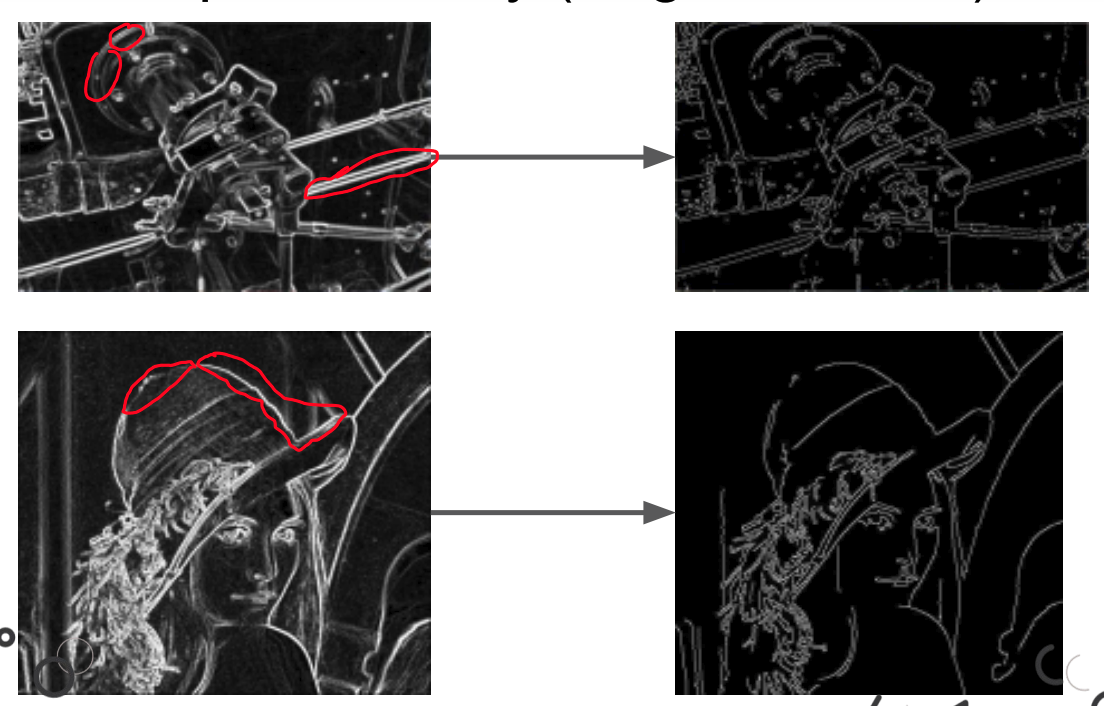
\includegraphics[scale=0.2]{canny0}
    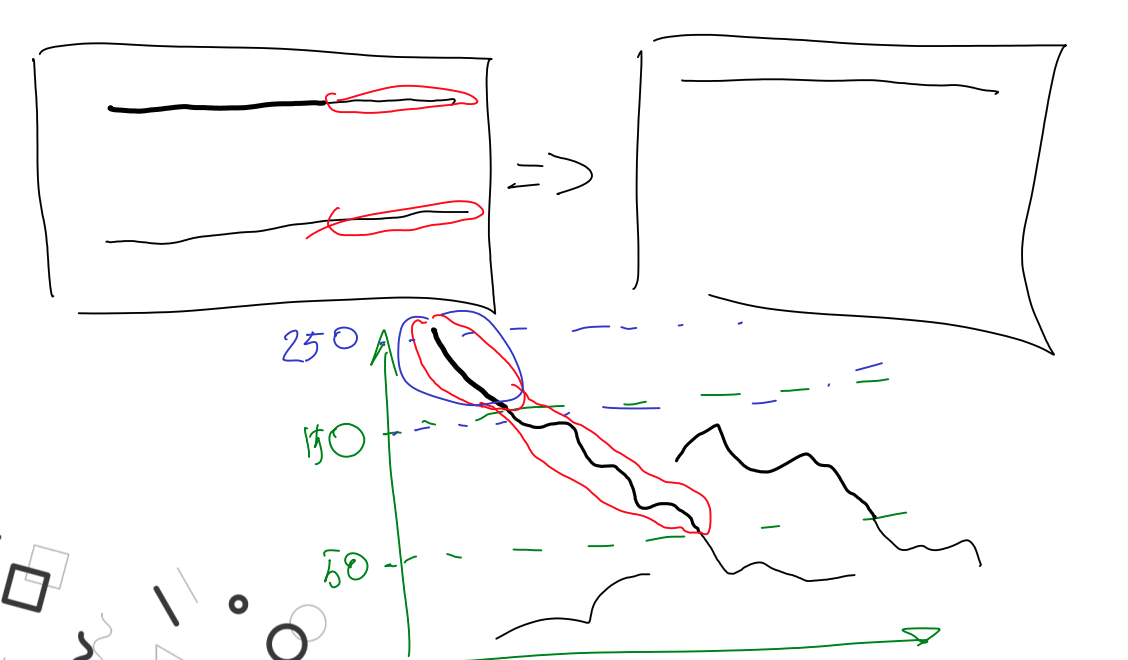
\includegraphics[scale=0.2]{canny}

\end{document}